\documentclass[utf8,xcolor=table]{beamer}

\usepackage[T2A]{fontenc}
\usepackage[utf8]{inputenc}
\usepackage[english,russian]{babel}
%\usepackage{tikz-uml}
%\usepackage{minted}

\mode<presentation>{
	\usetheme{CambridgeUS}
}

\renewcommand{\t}[1]{\ifmmode{\mathtt{#1}}\else{\texttt{#1}}\fi}

\title{Оффлайн-просмотр ленты ВКонтакте}
\author{Егор Суворов}
\institute[СПб АУ]{Практика, осень 2015--зима 2016}
\date[21.03.2016]{Понедельник, 21 марта 2016 года}

\setlength{\arrayrulewidth}{1pt}

\begin{document}

\begin{frame}
\titlepage
\end{frame}

\begin{frame}[t]{Мотивация}
	\begin{itemize}
		\item В мире много мест с плохой связью, где приходится чем-то занимать время
		\item Лента ВК занимает всё доступное время, но без интернета её не полистать
		\item Официальные клиенты не подходят:
			\begin{itemize}
				\item Могут выкидывать уже загруженные данные
				\item Не кэшируют страницы по приложенным к постам ссылкам
			\end{itemize}
	\end{itemize}
\end{frame}

\begin{frame}[t]{Задачи}
	\begin{itemize}
		\item Реализовать offline-first клиент ВК для просмотра ленты новостей
		\item Агрессивное кэширование, даже если какие-то фрагменты ленты остаются неподгруженными
		\item Автоматическое скачивание веб-страниц, на которые ссылаются записи (с зависимостями)
		\item Подгрузка ленты с любого места по запросу
	\end{itemize}
\end{frame}

\begin{frame}[t]{Пример разрыва ленты-1}
	\begin{center}
		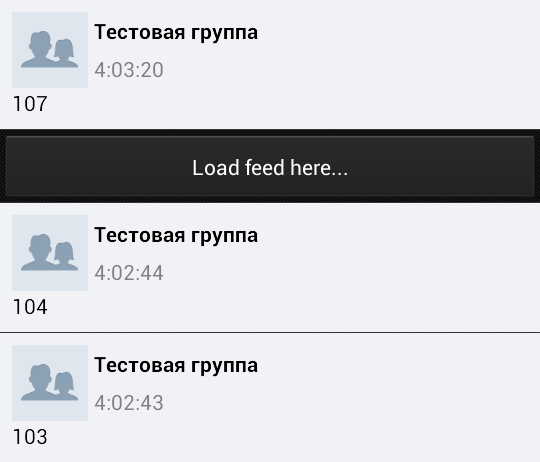
\includegraphics[scale=0.5]{a.png}
	\end{center}
\end{frame}
\begin{frame}[t]{Пример разрыва ленты-2}
	\begin{center}
		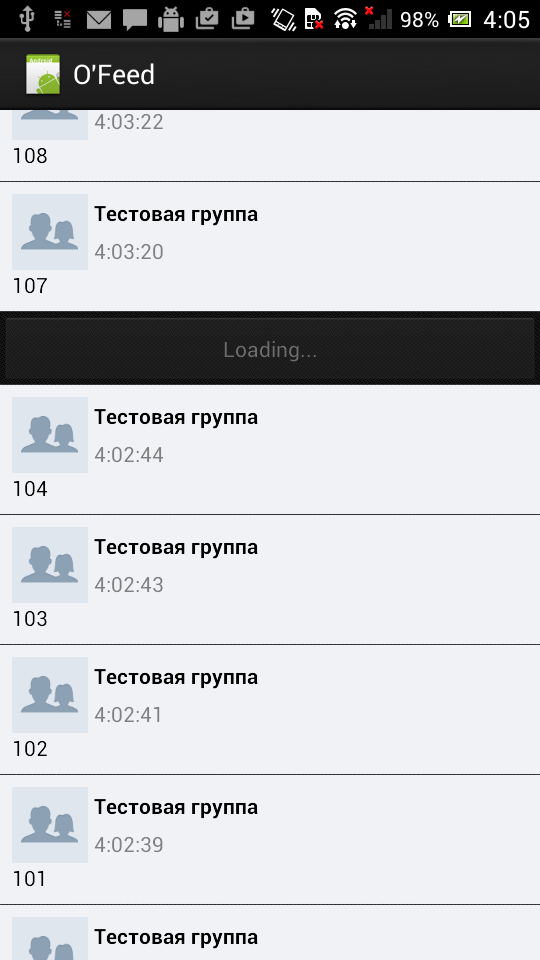
\includegraphics[scale=0.5]{b.png}
	\end{center}
\end{frame}
\begin{frame}[t]{Пример разрыва ленты-3}
	\begin{center}
		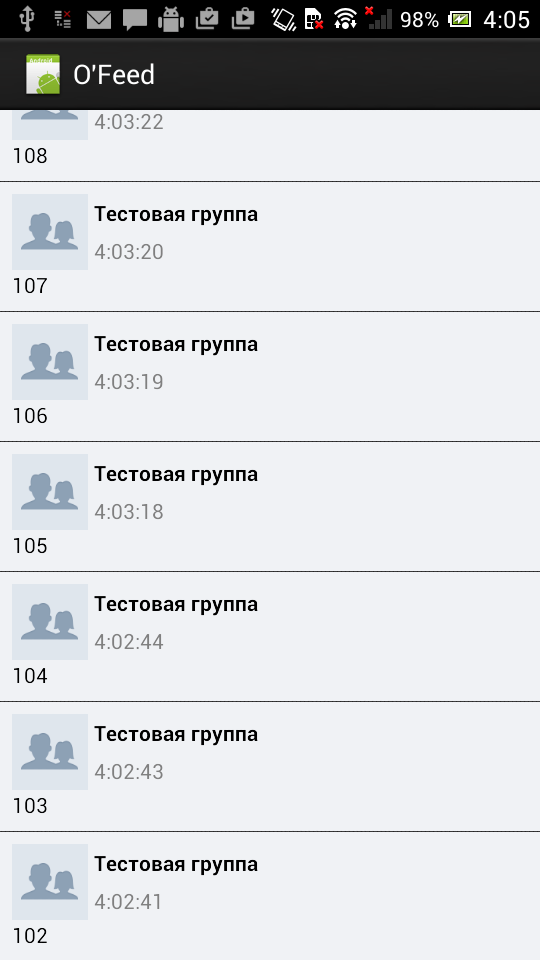
\includegraphics[scale=0.5]{c.png}
	\end{center}
\end{frame}

\begin{frame}[t]{Части приложения}
	Используются библиотеки:
	\begin{itemize}
		\item ORMLite "--- общение с базой данных (SQLite)
		\item JSoup "--- парсинг и изменение HTML
		\item VK Android Library "--- взаимодействие с VK API
	\end{itemize}
	Дописано самостоятельно:
	\begin{itemize}
		\item Java-обёртки для VK API, работающего с лентой новостей
		\item Модификация HMTL-страницы для offline-просмотра
	\end{itemize}
\end{frame}

\begin{frame}[t]{Сложные места}
	Удалось решить:
	\begin{itemize}
		\item Логика хранения фрагментированной ленты
		\item Адаптер для ListView для прокрутки длинных фрагментированных списков с возможностью догрузки в процессе
		\item Открытие HTML-файла с локального диска в браузере
	\end{itemize}
	Не реализовано:
	\begin{itemize}
		\item Поддержка всех типов вложений
		\item Комментарии и лайки
		\item Прозрачное управление кэшированием
		\item Обновление кэша
	\end{itemize}
\end{frame}

\begin{frame}[t]{Изменения с декабря}
	\begin{itemize}
		\item Функциональность не изменилась
		\item Добавлены автоматические проверки стиля кода при помощи checkstyle
		\item Проверка кода, дописанного к VK SDK, делается по другим правилам
	\end{itemize}
\end{frame}

\begin{frame}[t]{Ссылки}
  \begin{itemize}
  \item \href{mailto:egor_suvorov@mail.ru}{\t{egor\_suvorov@mail.ru}}
  \item \href{http://github.com/yeputons/ofeed/}{\t{github.com/yeputons/ofeed}}
  \item \href{http://yeputons.net/pub/ofeed.apk}{\t{yeputons.net/pub/ofeed.apk}}
  \end{itemize}
\end{frame}

\end{document}
